\documentclass[11pt]{article}
\usepackage{amsmath}
\usepackage[sc]{mathpazo} %Like Palatino with extensive math support
\usepackage{fullpage}
\usepackage[authoryear,sectionbib,sort]{natbib}
%\usepackage[square,sort,comma,numbers]{natbib}
\linespread{1.7}
\usepackage[utf8]{inputenc}
\usepackage{lineno}
\usepackage{titlesec}
\usepackage{xcolor}
\usepackage{graphicx}
\usepackage{placeins}
\usepackage{float}
\usepackage{subfigure}
\newcommand{\tom}[2]{{\color{red}{#1}}\footnote{\textit{\color{red}{#2}}}} 
\newcommand{\ali}[2]{{\color{blue}{#1}}\footnote{\textit{\color{blue}{#2}}}}  


\titleformat{\section}[block]{\Large\bfseries\filcenter}{\thesection}{1em}{}
\titleformat{\subsection}[block]{\Large\itshape\filcenter}{\thesubsection}{1em}{}
\titleformat{\subsubsection}[block]{\large\itshape}{\thesubsubsection}{1em}{}
\titleformat{\paragraph}[runin]{\itshape}{\theparagraph}{1em}{}[.]\renewcommand{\refname}{Literature Cited}


%%%%%%%%%%%%%%%%%%%%%
% Line numbering
%%%%%%%%%%%%%%%%%%%%%
%
% Please use line numbering with your initial submission and
% subsequent revisions. After acceptance, please turn line numbering
% off by adding percent signs to the lines %\usepackage{lineno} and
% to %\linenumbers{} and %\modulolinenumbers[3] below.
%
% To avoid line numbering being thrown off around math environments,
% the math environments have to be wrapped using
% \begin{linenomath*} and \end{linenomath*}
%
% (Thanks to Vlastimil Krivan for pointing this out to us!)

\title{Demographic consequences of partner diversity and turnover in a multi-species ant-plant mutualism}
% title suggestion, trying to move away from focus on IPM

\author{Alexandra Campbell$^{1,\dagger}$ \\ 
	Tom E.X. Miller$^{1,\ast}$}

\date{}

\begin{document}
	
	\maketitle
	
	\noindent{} 1. Program in Ecology and Evolutionary Biology, Department of BioSciences, Rice University, Houston, Texas 77005;
	
	\noindent{} $\dagger$ e-mail: amc49@rice.edu\\
	\noindent{} $\ast$ e-mail: tom.miller@rice.edu
	
	\bigskip
	
	\textit{Keywords}:  Integral Projection Model, \textit{Cylindropuntia imbricata}, population fitness, multi-species mutualism, complementarity, sampling effect, portfolio effect
	
	\bigskip
	
	\textit{Manuscript type}: Article.
	
	\bigskip
	
	\noindent{\footnotesize Prepared using the suggested \LaTeX{} template for \textit{Am.\ Nat.}}
	
\linenumbers{}
\modulolinenumbers[3]

\newpage{}

\section*{Abstract}
\tom{}{I think this is too long for Am Nat requirements. Also, use ``we''. I think you just pasted in an abstract that you used elsewhere, so I will work on this once you write a real abstract for the Am Nat paper.}
Mutualisms are widespread species interactions with diverse and dynamic consequences. 
They are considered more context dependent than other species interactions, meaning there are many different factors which change the outcomes of interactions between mutualists, including partner diversity. 
Partner diversity has become a central focus in the field of mutualisms, expanding previous work from primarily pairwise to multispecies mutualisms. 
It has been shown that pairwise studies are poor predictors of the effects of multispecies mutualistic interactions. 
The diversity of partners in a multi-species mutualism causes varied demographic effects on the population of the focal mutualist which can be explained by several mechanisms: portfolio effect, complementarity, and sampling effect. 

I use the plant-ant multi-species mutualism in which, the cactus \textit{Cylindropuntia imbracata} (tree cholla) pro- duce extrafloral nectar and the ants, \textit{Crematogaster opuntiae}, \textit{Liometopum apiculatum}, \textit{Forelius pruinosus}, and rarer species, provide defense from various herbivores and seed predators. 
I used 18 years of data collected from plant demographic censuses, which includes data such as size, survival, reproductive status, flowers produced, and ant partner for all plants in 8 30$\times$30 m plots at the Sevilleta National Wildlife Refuge in central New Mexico. 
With this data I parameterize a series of Bayesian hierarchical generalized linear vital rate models to determine the impacts of different partners on the focal mutualists. 
I found that different ant partners had different impacts on the vital rates of the tree cholla. 
Specifically, \textit{C. opuntiae} tended plants had advantages in both growth and survival when small, and large \textit{L. apiculatum} tended plants had floral viability advantages. 
With these models I constructed an Integral Projection Model in which I could vary the presence of each partner, creating different “diversity scenarios”, to determine under which diversity scenario the focal mutualist experienced the highest plant fitness, and which mechanism(s) may explain the effects of partner diversity. 
I found that the all scenarios which included the partner \textit{L. apiculatum} resulted in the highest possible fitness for the tree cholla. 
Results further suggest that diversity benefits in this system are driven by sampling effect , meaning \textit{L. apiculatum} ants are the "best`` partner.
I also found that partner diversity benefits the focal mutualist in this system in the form of portfolio effect by buffering the tree cholla from the effects of inter-annual variation. 
This study highlights how partner diversity can increase the overall benefits a focal mutualist receives. 
It also highlights the importance of a mechanistic understanding to explain the benefits of this diversity across systems.

\newpage{}
\section*{Introduction}
Mutualisms are species interactions where all participants receive net benefits, leading to higher individual fitness and increased population growth rates. 
They are widespread species interactions \citep{Bronstein1994,Chamberlain2014,Frederickson2013,Axelrod1981,Leigh2010} but can deteriorate into commensalism or parasitism under conditions that elevate costs or dampen benefits \citep{Rodriguez-Rodriguez2017,Song2020,Mandyam2014,Thrall2007, Bahia2022}.
Mutualisms are considered more context dependent than other species interactions \citep{Chamberlain2014,Frederickson2013}, meaning the magnitude and sign of interaction strength are often determined by environmental conditions and species' identities \citep{Noe1994,Leigh2010}.

Mutualism is defined at the level of a species pair (+/+) but these interactions are embedded within multi-species communities, and growing evidence suggests that pairwise interactions are poor predictors of the net effects of multi-species mutualism \citep{Afkhami2014,Palmer2010,Bascompte2009,Dattilo2014}. 
A focal mutualist may interact with multiple guilds of partner types (e.g., plants that interact with pollinators, seed dispersers, soil microbes, and ant defenders) or with multiple partner species within the same guild (e.g., plants visited by multiple pollinator species). 
Within a mutualist guild, partner species often differ in the amount or type of goods or services they provide, making partner identity an important source of contingency in mutualism \citep{Stanton2003}. 
Whether and how partner diversity modifies the demographic effects of mutualistic interactions remain open questions within relevance in \tom{applied settings}{would be good if you could find another applied example to cite here} \citep{rogers2014}.

There are multiple mechanisms by which partner diversity can influence the net benefits accrued by a focal mutualist, mirroring the mechanisms by which, at a larger scale of organization, biodiversity can influence ecosystem function \cite{Yeung2006,Barrett2015,Ushio2020}. 
First, when there is a hierarchy of fitness effects (a consistent ranking of best to worst mutualists), a more diverse sample of the partner community may be more likely to include the best partner \cite{Frederickson2013}.
This can lead to an apparent benefit of diversity driven by a sampling effect \cite{Batstone2018} -- but there is no benefit of diversity \emph{per se}, only better and worse partners. 
If partner associations are mutually exclusive (a focal mutualist may engage with only one partner at a time), then partner diversity may impose opportunity costs, leading to negative effects of a diverse mutualist assemblage relative to exclusive association with the single best partner \citep{Miller2007}. 
Second, even within a single mutualist guild, the benefits conferred by alternative partner species can vary in type and not just degree \cite{Stachowicz2005,Bronstein2006,Stanton2003}. 
This can lead to a positive effect of partner diversity through complementarity of alternative functions \cite{Batstone2018}. 
Interference or synergies between partners can make their combined effect different than the expected from the sum of complementary functions \cite{Afkhami2014}. 
Third, partner species can have species-specific responses to environmental variation, either spatially \citep{Ollerton2006} or temporally \citep{Alarcon2008}. 
Multiple partners can therefore act as a 'portfolio' that stabilizes fitness benefits across spatial or temporal heterogeneity, leading to positive effects of partner diversity through the portfolio effect \cite{Batstone2018,Lazaro2022,Horvitz1990}. 

Partner diversity can have different effects depending on whether partners are present all at once or sequentially (partner turnover) \citep{Djieto-Lordon2005, Ness2006, Bruna2014,Barrett2015,Ushio2020,Dattilo2014}. 
Sequential associations are likely when alternative partners engage in interference competition for access to a shared mutualist \cite{Kiers2003,Batstone2018,Tgaard2015,Wulff2008}. 
Turnover can happen at different timescales, from minutes to years \citep{Oliveira1999,Horvitz1986}. 
The frequency of partner turnover can impact the level of benefits received by the focal mutualist, particularly if the benefits continue to accumulate with successive turnover (e.g., when sequential partners provide complementary functions) or if they saturate over time \citep{Sachs2004,Fiala1994}.
Directionality of turnover can also influence effects of partner diversity if partner identity changes consistently across ontogeny of a focal mutualist \citep{Fonseca2003,Noe1994,Dejean2008}.
For example, plant susceptibility to enemies can change across life stages \citep{Boege2005,Barton2010}, so the benefits of defensive mutualism with ants are greatest when more defensive partner species align with more vulnerable life stages \citep{Djieto-Lordon2005,Dejean2008}.

Defensive ant-plant mutualisms -- where plants provide food and/or housing to ants that in turn defend them from enemies -- are widespread interactions that offer valuable model systems for the ecology and evolution of mutualism \citep{Bronstein1998, Bronstein2006}. 
Extrafloral nectar (EFN) -bearing plants can serve as dietary resources that promote ant abundance and colony size \citep{Byk2011, Ness2009, Ness2006, Donald2022}.
Presence of defensive ant partners is often linked to reductions in herbivory  \citep{Trager2010, Rudgers2004} and demographic advantages for the plant partner \citep{Baez2016}.
Defensive ant-plant mutualisms are commonly multi-species, where a guild of ant partner species share, and often compete for, a plant mutualist \citep{Bronstein1998, Beattie1985, Trager2010, Agrawal1998}.
Ant partners can vary in their ability to deter herbivores \citep{Bruna2014}, and visitation by low quality ant partners can prevent visitation by higher quality partners, consequently causing a reduction in fitness through missed opportunity costs \citep{Fraser2001, Frederickson2005}.
Susceptibility to herbivory can also vary significantly throughout the life stages of the plant \citep{Boege2005}, suggesting that the order and timing of successive partners is important to the fitness impacts of the combined partner guild \citep{Barton2010, Boege2005, Fonseca2003}.
Herbivore identity and pressure can vary inter-annually \cite{Wetzel2023}, much like mutualist identity and presence, meaning the threat plants face can vary just as much as the protection they receive due to temporal stochasticity. 
Previous studies have investigated how ant partner diversity affects plant fitness \citep{Palmer2010,Afkhami2014,Fiala1994,Gaume1998,Dattilo2014,Ludka2015}
However, little is known about the combined effects of partner identity, directional partner turnover, and temporal stochasticity, particularly because the necessary long-term data are rarely available. 
	
This study examined the consequences of partner diversity in a food-for-protection mutualism between the tree cholla cactus (\textit{Cylindriopuntia imbricata}), a long-lived EFN-bearing plant, and multiple species of ant partners.
Previous studies have shown that herbivory by specialized insect herbivores negatively affects plant fitness \cite{Miller2009}, and ant defense reduces herbivore damage \cite{Miller2007}. 
Tree cholla are tended by two common ant species (\textit{Liometopum apiculatum} and \textit{Crematogaster opuntiae}) and several additional rarer species, all of which collect EFN during foraging visits but their colonies are ground-nesting and not housed by the plants. 
These ant species locally co-occur but individual plants are typically tended by only one species that patrols the plant around-the-clock and maintains control of the plant's nectar resources for an entire growing season \citep{Ohm2014, Donald2022}. 
Switches between partner species, or between vacancy and ant occupancy, commonly occur from one growing season to the next \citep{Miller2007}. 
Prior experiments suggested a hierarchy of mutualist quality, with \textit{Liometopum apiculatum} providing strong anti-herbivore defense and \textit{Crematogaster opuntiae} having net negative effects because herbivore deterrence is outweighed by deterrence of pollinators \citep{Miller2007,Ohm2014}. 
However, previous studies in this system focused on single life stages (adult plants) or vital rates (seed production) and did not integrate the demographic effects of ant defense across the life cycle, which may be essential for understanding net fitness effects \citep[e.g.,][]{Palmer2010}. 
To our knowledge no previous study has incorporated inter-annual stochasticity into models of ant-plant dynamics, which limits our understanding of diversity benefits that may arise through the portfolio effect. 

We used a unique long-term data set that allows us to explore mutualistic associations with multiple partner species, longitudinal turnover in partner identity at the individual level, and how the demographic effects of alternative partner species varied across plant size structure and nearly 20 years of inter-annual fluctuations. 
We used this observational data set of ant-plant associations, informed by previous ant exclusion experiments, to ask whether and through which mechanism(s) partner diversity affects the fitness benefits of ant visitation for the focal plant partner. 
Specifically, we asked:
	\begin{enumerate}	
		\item{What are the demographic effects of association with alternative partners and how do these effects fluctuate across years?}
		\item{What are the frequency and direction of partner turnover across the plant life cycle?}	
		\item{What is the net effect of partner diversity on plant fitness, and what mechanism(s) explain(s) this effect?}
	\end{enumerate}
We used a hierarchical Bayesian statistical approach to estimate demographic vital rates for hosts in different states of ant occupancy and to quantify state-dependent partner turnover from the long-term data. 
We then used a stochastic, multi-state integral projection model (IPM) that combines diverse effects on vital rates and pathways of partner turnover to quantify effects of partner diversity on plant fitness. 


\section*{Methods}
\subsection*{Study System}
  
This study was conducted in the Los Pi$\tilde{n}$os mountains, a small mountain chain located on the Sevilleta National Wildlife Refuge, a Long-term Ecological Research site (SEV-LTER) in central New Mexico, USA.
This is an area characterized by steep, rocky slopes, and perennial vegetation including grasses (\textit{Bouteloua eriopoda} and \textit{B. gracilis}), yuccas, cacti, and junipers. 
Tree cholla cacti are common in high Chihuahuan desert habitats, with their native range spanning the southwestern USA \citep{Benson1982}. 
These arborescent plants produce cylindrical segments with large spines. 
In the growing season (May to August in New Mexico), the plants initiate new vegetative segments and flower buds at the ends of existing segments. 
While most plants produce new segments every season, only those which are reproductively mature produce flower buds. 
%Tree cholla generally reach at least 9 years of age before beginning to reproduce \citep{Ohm2014}.
Like other EFN-bearing cacti, tree cholla secrete nectar from specialized glands on young vegetative segments and flower buds \citep{Ness2006,Oliveira1999}. 
Flower buds produce more and higher-quality EFN than vegetative segments, making reproductive cholla valuable mutualist partners \citep{Miller2014}. 
%Smaller cholla produce little to no EFN, so larger cholla, especially flowering individuals, are generally more highly tended. 

Tree cholla EFN is harvested by various ant species. 
At SEV-LTER, cholla are visited primarily by two species of ground-nesting ants, \textit{Crematogaster opuntiae} and \textit{Liometopum apiculatum}, as well as other rarer species, including \textit{Forelius pruinosus} and unidentified species in the genera \textit{Aphaenogaster} and \textit{Camponotus}.
\textit{L. apiculatum} are the most frequent visitors with $25\% - 60\%$ of tree cholla tended by these ants, followed by \textit{C. opuntiae} visiting between $5\% - 20\%$ of cacti depending on the year \citep{Donald2022}. 
Between $ 30\% - 80\%$ of cacti remain vacant in any given year. 
Workers of different species rarely co-occur on individual plants, likely due to interspecific competition \citep{Miller2007}: staged introductions of \textit{C. opuntiae} to \textit{L. apiculatum}-tended plants, and vice versa, provoke aggressive responses by residents (A. Cambpell, \textit{personal observation}).
%Each cholla is visited by a single ant species for the duration of a season, and the species of the visitors can change from one season to the next. 
In Fall, tree cholla stop producing EFN and the ants vacate until the next growing season. 

Multiple insect herbivores and seed predators specialize on tree cholla \citep{Mann1969}. 
The Cerambycid beetle \textit{Moneilema appressum} and a weevil (Curculionidae) of the genus \textit{Gerstaekeria} feed on vegetative and reproductive structures as adults and their larvae feed internally. 
A cactus bug, \textit{Narnia pallidicornis} (Hemiptera: Coreidae), feeds on all cholla parts with a preference for the reproductive structures \citep{Miller2006}.
A seed predator, \textit{Cahela ponderosella} (Lepidoptera: Pyralidae), oviposits in open flowers and larvae eat seeds in developing fruits. 
These predators can have significant negative impacts on plant fitness of and depress population growth \citep{Miller2009}.
Prior experiments showed that ant-tended tree cholla experience less herbivory and seed predation than plants from which ants were excluded \citep{Miller2007,Ohm2014}. 

\subsection*{Data Collection}
This study is based on long-term demographic data spanning 2004 to 2023 at SEV-LTER. 
From 2004 to 2008, we censused 134 plants distributed across three spatial blocks. 
This initial census group was discontinued in 2009, when we established six 30 $\times$ 30-meter plots and tagged all tree cholla within those plots. 
Two additional 30 $\times$ 30-meter plots were added in 2011, and this group of eight plots has since been censused annually through 2023 (with the exception of 2020 due to the pandemic shutdown). 
For all plants, in May or early June of each year we recorded plant survival since the last survey and, for survivors, we recorded height (cm), maximum crown width (cm), and crown width perpendicular to the maximum (cm).
Size measurements were used to calculate plant volume ($cm^3$) based on the volume of an elliptical cone. 
We recorded reproductive effort as counts of viable and aborted flowerbuds. 
We recorded the ant species present (or vacancy if no ants present).
Occurrences of more than one ant species on one plant were rare (less than 5\% of observations), and for the purpose of this analysis we classified the plant as being occupied by the more abundant species. 
Plots were searched for new recruits each year, and these were added to the census.
In total, the data set included 1141 unique individuals and \tom{19 plant-year observations}{It is 19 years but the number of plant-year observations should be the total number of rows in the data set}. 
%These data were used to fit vital rate models (survival, growth, reproduction) as functions of plant size and ant occupancy state. 

We used additional, smaller data sets from previously published studies to estimate seed and seed bank parameters. 
Ohm et al. \citep{Ohm2014} provide data on the number of seeds per fruit for plants tended by \textit{L. apiculatum}, \textit{C. opuntiae}, or no ants (experimental exclusion). 
Miller et al. \citep{Miller2009} provide data on seed entry to the seed bank and seedling germination and survival rates. 


\subsection*{Multi-state Integral Projection Model}
Integral Projection Models describe population dynamics in discrete time, with functions that relate vital rates to continuous state variables. 
While IPMs are a natural choice for populations with continuous size structure, they can also be modified to accommodate a combination of continuous and discrete state variables, as we do here. 
We constructed a multi-state IPM that stitches together population structure associated with plant size and ant state, allowing us to determine the individual fitness effects of each ant species and the composite effects of multiple partners, with their transition dynamics modeled explictly. 

Given the low frequency of ant species other than \textit{L. apiculatum} and \textit{C. opuntiae} (7.78\% of observed ants) we combined observations of all other ants into an ``other'' category, such that our models included four possible ant states: vacant, \textit{L. apiculatum}, \textit{C. opuntiae}, and ``other''. 
The ``other'' category was made of unidentified ant species (2.8\% of observed ants), unknown species belonging to the geni \textit{Aphenogaster} (0.4\%),  \textit{Camponotus} (0.9\%),  \textit{Tetramorium} (0.02\%), \textit{Brachymyrmer} (0.02\%), a honeypot ant (0.08\%), and \textit{Forelius pruinosus} (3.5\%).
Ant state is included as a predictor variable in sub-models where there are biologically realistic pathways through which ants could impact the outcome of that process. 
For example, ant partners defend cacti from herbivores, and prior experimental work indicates that ant tending can reduce vegetative tissue loss and floral abortion.
Therefore, ant state was included in sub-models for survival, growth, and flowerbud viability. 
In contrast, we have no reason to expect that ant tending can directly influence the probability of flowering and flowerbud production, independently of its influence on plant size. 
Therefore, these sub-models included plant size but not ant state as predictor variables. 

Following previous studies, we modeled the tree cholla life cycle using continuously size-structured plants where $n(x,a)_{t}$ gives the number of plants of size $x$  and ant state $a$ in year $t$, plus two discrete seed banks ($B^1_{t}$ and $B^2_{t}$) corresponding to 1 and 2-year old seeds. 
Seed bank dynamics are given by:

\begin{linenomath*}
	$$
	B^1_{t+1} = \delta \sum_{a=1}^{A} \int_L^U  \kappa(a') P(x;\pmb{\tau^P}) F(x;\pmb{\tau^F}) V(a;\pmb{\tau^V_{a}}) n(x,a)_{t} dx \\
	$$
	$$
	B^2_{t+1} =  (1 - \gamma_1)B^1_{t}\\
	$$
\end{linenomath*}

\noindent In these equations $x$ and $x'$ indicate the size of a plant in years $t$ and $t+1$ respectively, $a$ and $a'$ indicate the ant partner of a plant in years $t$ and $t+1$.
Functions $P(x;\pmb{\tau^P})$ and $F(x;\pmb{\tau^F})$ give the probability of flowering in year $t$ and the number of flowerbuds produced in year $t$, respectively, by plants of size $x$. 
The proportion of flowerbuds that remain viable through fruit set ($V(a;\pmb{\tau^V_{a}})$) and the number of seeds per fruit ($\kappa(a)$) are dependent on ant state $a$ but not size. 
The vector $\pmb{\tau}$ gives year-specific deviates (with mean zero) and appears in functions for which we can estimate temporal stochasticity from the long-term data; superscripts indicate the corresponding vital rate and subscripts indicate that deviates are specific to plants in ant state $a$ and year.
Seed production is integrated over the size distribution, from the lower $L$ to upper $U$ size limits, and summed over all possible ant states ($A=4$) giving total seed production. 
Seeds are multiplied by the probability of seed dispersal and survival ($\delta$) to give the number of seeds that enter the one-year old seed bank. 
Plants can recruit out of the year-one seed bank with probability $\gamma_1$ or transition to the two-year seed bank with a probability of $1 - \gamma_1$. 
Seeds in the two-year seed bank are assumed to either germinate with probability $\gamma_2$ or die. 

For the above-ground part of the life cycle, the number of plants of size $x'$ and ant state $a'$ in year $t+1$ ($n(x',a')_{t+1}$) is given by survival/growth transitions from size $x$ and ant state $a$ in year $t$, plus germination out of the seed banks:
\begin{linenomath*}
	$$
	n(x',a')_{t+1} = (\gamma_1 B^1_{t} + \gamma_2 B^2_{t} ) \eta(x') \omega \rho_{0}(a')  + \\
	$$
	$$
	\sum_{a=1}^{A} \int_L^U S(x,a;\pmb{\tau^S_{a}}) G(x',x,a;\pmb{\tau^G_{a}}) \rho(x,a,a';\pmb{\tau^{\epsilon}}) n(x,a)_t dx \\
	$$
\end{linenomath*}

\noindent The first term estimates the number of individuals recruiting from a one or two-year seed bank to a plant of size $x'$ and ant state $a'$ based on the recruit size distribution $\eta(x')$ and the probability of seedling survival ($\omega$) from germination (late summer) to the census (May).
This term is multiplied by $\rho_{0}(a')$, which gives the probability that a new recruit has ant state $a'$ at its first appearance in our census ($\sum_{a'}^{A}\rho_{0}(a')=1$). 
The second term represents all possible transitions from size $x$ and ant $a$ to size $x'$ and ant $a'$, conditioned on survival. 
Survival from initial size $x$ ($S(x,a;\pmb{\tau^S_{a}})$) and growth from size $x$ to $x'$ ($G(x',x,a;\pmb{\tau^G_{a}})$) are both dependent on initial size and ant state. 
As above, these functions include inter-annual variability through year-specific deviates that can vary by ant state ($\pmb{\tau_{a}}$). 
Ant transition function $\rho(a',a,x;\pmb{\tau^{\rho}})$ gives the probability that an individual transitions from ant state $a$ to $a'$ in the next census, conditional on initial size $x$. 
This function includes inter-annual variability through year-specific intercepts which are consistent across ant states ($\pmb{\tau^\rho}$).

\subsection*{Statistical modeling and parameter estimation}
We parameterized the IPM using a series of generalized linear mixed models (GLMMs) in a hierarchical Bayesian framework to serve as vital rate sub-models. 
Vital rate models included spatial and temporal random effects associated with plot and year variation, respectively, and included plant size ($log(cm^3)$; $x,x'$), ant partner state ($a,a'$), or both as fixed-effect predictor variables. 
In addition to vital rate models describing plant demographic performance, we also fit a sub-model to predict transition between ant states conditional on plant size and previous ant state. 
All models were fit using R version 4.2.2 and Rstan package (\cite{Rstancite, Rcite}).
Unless otherwise mentioned, all used vague priors. 

The vital rate models take the form of the function:
$$ f(\mu) = \beta_0 + \beta_1 x + ... + u + w $$
\noindent where $u \sim N(0,\sigma_{yr }^{2})$ is the year random effect with year specific deviates of $\sigma_{yr}$ (which parameterizes the $\tau$ vector), and $w \sim N(0,\sigma_{plot}^{2})$ is the plot random effect with plot specific variance of $\sigma_{plot}$. 
Some models deviate from this general model, which will be specified below.

\paragraph{Growth}
The growth sub-model ($G(x',x,a;\pmb{\tau^G_{a}})$) gives the probability of future size given the fixed effects of previous size $x$ and previous ant partner $a$ and random effects of plot $w$ and year $u$ which interacts with ant state $a$. 
We fit this model to the size in year $t+1$ ($y^G$) using the location-scale parameterization of the student $t$ distribution and the identity link function, because in preliminary analyses we found that size transition data were more fat-tailed than a Gaussian distribution could accommodate. 
$$y^G \sim Student T(\hat{\nu},\hat{G},\hat{\sigma}) $$
Student $t$ distributions are dependent on three parameters, $\hat{\nu}$,  $\hat{G}$, and $\hat{\sigma}$.
$\hat{G}$ is the mean of the distribution, and in our case is expressed as a second-order polynomial with ant-size interactions because  preliminary analysis found this was a better fit to slightly concave data. 
$\hat{\nu}$ is the shape parameter which determines how thin the tails of the distribution are.
$\hat{\sigma}$ is the scale parameter which determines how wide the distribution is. 
Both $\hat{\nu}$ and $\hat{\nu}$ are size dependent because preliminary analyses revealed that there was size dependence in both variance and kurtosis.
%$$\hat{G} = \beta_{0}^{G} + \beta_{1}^{G}  x  + \beta_{2}^{G}  a + \beta_{3}^{G}  x  a  + \beta_{4}^{G}  x^2 + \beta_{5}^{G}  a  x^2 + u + w $$
$$\hat{\sigma} = \beta_{0}^{\sigma} + \beta_{1}^{\sigma}  x $$
$$\hat{\nu} = \beta_{0}^{\nu} + \beta_{1}^{\nu}  x $$


\paragraph{Survival}
The survival model ($S(a,x;\pmb{\tau_{a}^{S}})$) estimates the probability of survival from year $t$ to year $t+1$, with fixed effects of the previous size of the cholla $x$ and ant partner $a$ in year $t$ and random effects of plot $w$ and year $u$ which interacts with ant state $a$.
We fit this model to the survival data $y^S$  using a Bernoulli distribution and the logit link function
$y^S \sim Bern(\hat{S})$.
%$$logit(\hat{S}) = \beta_{0}^{S} + \beta_{1}^{S}  x + \beta_{2}^{S}  a + \beta_{3}^{S}  x  a + u + w$$

\paragraph{Reproduction}
The reproduction model ($P(x';\pmb{\tau^{P}})$) estimates the probability of reproducing in year $t+1$, with fixed effects for the size $x'$ in year $t+1$ and random effects of plot $w$ and year $u$.
We fit this model to the reproductive data $y^R$ using a Bernoulli distribution and a logit link function:
$$y^P \sim Bern(\hat{P})$$
%$$logit(\hat{P} = \beta_{0}^{P} + \beta_{1}^{P} \times x' + u + w)$$


\paragraph{No. Flowers}
The total flowers model ($F(x';\pmb{\tau^{F}})$) estimates the total flowers produced by a plant in year $t+1$, with fixed effects of size $x'$ in year $t+1$ and random effects of plot $w$ and year $u$. 
We fit this model to flowerbud count data $y^F$ using a zero-truncated negative binomial distribution with a log transformation:
$$y^{F} \sim 0 Truncated Negative Binom(\hat{F},\hat{\phi})$$
%$$log(\hat{F}) = \beta_{0}^{F} + \beta_{1}^{F} \times x' + u + w$$
$$log(\hat{\phi}) = \beta_{0}^{\phi}$$


\paragraph{Flowerbud viability}
The viability model ($V(a;\pmb{\tau^{V}_{a}})$) estimates theproportion of flowers produced by a plant which are viable (not aborted) in year $t+1$, with fixed effects of ant partner $a$ in year $t$ and random effects of plot $w$ and year $u$ which interacts with ant state $a$.
We fit this model to floral abortion data $y^V$ using a Binomial distribution and a logit link function:
$$y^{V} \sim Binom(\hat{V})$$
%$$logit(\hat{V}) = \beta_{0}^{V} \times a + u + w$$


\paragraph{Seeds Per Fruit}
With data\cite{Miller2006}, we fit a model for the number of seeds produced by every fruit on a cholla ($\kappa(a')$) in year $t+1$ based on the ant partner $a'$ in year $t+1$.
We fit this model to seed data $y^{\kappa}$ using a Negative Binomial distribution and the log link function: 
$$y^{\kappa} \sim  Negative Binomial(\hat{\kappa},\hat{\phi})$$
%$$ \hat{\kappa } = \beta_{0}^{\kappa} \times a'$$
$$\hat{\phi} = \beta_{0}^{\phi}$$
The data used for this model did not include data on ants in the ``other" category, so we used the data from vacant plants to parameterize seeds per flower for plants with ``other" ants in the IPM.

\paragraph{Ant Transitions}
The ant transition model ($\epsilon(x,a,a';\pmb{\tau^{\epsilon}})$) estimates the probability of a cactus being visited by an ant partner $a'$, with fixed effects of the previous size $x$  and the previous ant partner $a$  in year $t$ and random effects of plot $w$ and year $u$.
We fit this model to ant partner data from year $t+1$ $a'$ using a multinomial distribution with a logit link function: 
$$y^{\epsilon} ~ Multinomial(\hat{\epsilon})$$
%$$logit(\epsilon) = \beta_{0}^{\epsilon} + \beta_{1}^{\epsilon} \times x + \beta_{2}^{\epsilon} \times a + u$$


\paragraph{Recruit Size Distribution}
%The recruit size model ($n(x',a')$) estimates the size distribution of all recruits } from a given year $t+1$, with no fixed or random effects. 
We fit this model to recruit size data $y^{\eta}$ using a Normal distribution with the identity link function: 
$$y^{\eta} ~\sim N(\hat{\eta},\hat{\sigma})$$
%$$\hat{\eta} = \beta_{0}^{\eta}$$
where $\hat{\sigma}$ is estimated with a non-informative prior. 

\paragraph{Germination}
With germination data \cite{Miller2007}, we fit two models for the probability of germinating from the first year seedbank ($\gamma_1$) or the second year seedbank ($\gamma_2$) in year $t+1$, with no fixed or random effects.
These models were fit to germination data $y^{\gamma_1}, y^{\gamma_2}$  using the binomial distribution with logit link functions:
$$y^{\gamma_1} \sim Binomial(\hat{\gamma_1})$$
$$y^{\gamma_2} \sim Binomial(\hat{\gamma_2})$$
%$$logit(\hat{\gamma_1}) = \beta_{0}^{\gamma_1}$$
%$$logit(\hat{\gamma_2}) = \beta_{0}^{\gamma_2}$$

\paragraph{Pre-Census Survival}
With recruit census data \cite{Miller2006}, we fit a model for the probability of a seedling (which germinates in early Fall) surviving to when we census in May ($\delta$) of year $t+1$ (accounting for missed mortality events), with fixed effects of the previous size $x$ and random effects of the transect $m$.
We fit this model to pre-census survival data $y^{\delta}$ using a Bernoulli distribution with a logit link function: 
$$y^{\delta} ~ Bern(\hat{\delta})$$
%$$logit(\hat{\delta}) = \beta_{0}^{\delta} + m$$
 where $m \sim N(0, \sigma_{transect}^2)$ is the random effect of transect where the recruited individual was analyzed for survival.

\paragraph{Parameter estimation}
To obtain posterior estimates of the demographic parameters, we fit models using Markov chain Monte Carlo (MCMC) simulations via STAN run through version 4.0.2 of R \cite{Rcite,Rstancite}. 
For each model, we obtained three chains of 10,000 iterations, each with randomly chosen initial conditions. 
The first 1,500 iterations were discarded. 
We did not thin the chains, thus all samples were retained following burn-in. 
We assessed parameter convergence between and within chains (Figures \ref{fig:Surv_post} -- \ref{fig:Pre_Surv_post} b). 
To assess the overall model fit we carried out posterior predictive checks to examine how well the fitted model can generate simulated data similar to the real data (Figures \ref{fig:Surv_post} -- \ref{fig:Pre_Surv_post} a).
All estimated parameters are available in Table \ref{tab:Params}.

\subsection*{IPM Analysis}
We constructed two stochastic IPMs in order to simulate ant combinations that don’t exist in real life with two different versions of environmental variation.
The first is referred to as the stochastic IPM, in which we include random annual variation in the model and allow each ant partner to respond distinctly to annual variation. 
The second is referred to as the stochastic null IPM, in which we include random annual variation in the model, but force each ant partner to respond in the same way to annual variation. 
By analyzing the stochastic model we can estimate the fitness of the cholla under these simulated combinations.
By comparing the stochastic model to the stochastic null model we can identify what mechanisms may explain differences in cholla fitness with different ant partners. 
In this section I first explain how a simple deterministic IPM is developed before diving into how we created our more complex stochastic and stochastic null models. 

Analyzing an IPM requires discretizing the continuous IPM kernel into an approximating matrix. 
Size variable $x$ is discretized into $b$ bins, resulting in a $b \times b$ matrix.
In our model there is additional complexity in the form of transitions between ant partners, leading to a matrix size of $A b \times A b$ where $A$ is the number of unique combinations of $a$ and $a'$ (how many possible ant transitions there are).
Our model also has two additional discrete states (year one and year two seed banks) leading to a final matrix size of $A(b+2) \times A(b+2)$.
We used $b = 200$ bins after stability analysis to determine how many bins were needed to consistently estimate the same lambda.
We extend the integration limits $L$ and $U$ (the lowest and highest size values observed) to avoid unintentional eviction \cite{Williams2012}.

Traditionally, in a bayesian IPM, rather than having one set of parameters to populate an approximating matrix and estimate population fitness ($\lambda$), we use 1,000 draws from the posterior distributions of our bayesian statistical models to populate 1,000 approximating matrix and estimate a 1,000 element distribution for $\lambda$.
After preliminary stability analysis we found that 1,000 random posterior draws leads to the same estimate of $\lambda$ as any greater number of posterior draws.
In a stochastic bayesian IPM, the estimation of each individual $\lambda$ in the distribution comes from a geometric mean of many values. 
Rather than a single approximating matrix for each value of $\lambda$, we take the geometric mean of 500 approximating matricies with year-ant-specific effects, resulting in a stochastic version of populationfitness ($\lambda_{S}$).
These year-ant-specific effects are calculated as random effects for each unique combination of year and ant species included in our data. 
While we do not have data on how the ant species actually fluctuate annually, we are able to measure how the effects of the ant species on plants fluctuate annually.
Each of these 500 approximating matricies have the same draw from the posterior distribution, but are assigned the year-ant-specific effects of a random year of our data (year-ant-specific effects are sampled randomly with replacement).
We chose to use 500 year-specific values, because our $\lambda_{S}$ calculations stablilized after 500 year-specific values. 
To calculate a single $\lambda_{S}$ for these 500 year-ant-specific estimates, we take the geometric mean of the \ali{500 dominant eigenvalues}{OK, I am not positive this is correct, but I have forgotten how to correctly describe it. Can we talk through this sentence?} for a single stochastic $\lambda_{S}$.
This process is repeated for each of the 1,000 random posterior draws, leading to a distribution of 1,000 stochastic $\lambda_{S}$ values. 
To calculate the stochastic null bayesian IPM we use the exact same process, but the year-specific values used to calculate the stochastic null $\lambda_{SN}$ are not ant specific, forcing all ant species to have the same effects on their cactus partners in response to environmental variation.

In the both versions of our IPM, this process is repeated separately for every combination of ant partners: complete vacancy; \textit{C. opuntiae} and vacancy; other and vacancy; \textit{L. apiculatum}, \textit{C. opuntiae}, and vacancy, \textit{L. apiculatum}, other, and vacancy; \textit{C. opuntiae}, other, and vacancy; and all ant partners and vacancy.
Each partner scenario includes vacancy in addition to the combination of partners being analyzed for added realism because we have never observed a population of cacti in which all are occupied. 

We can compare the distributions of $\lambda_{S}$ in many ways, but have chosen two moments in particular: the means and the proportion of each distribution that is greater than another.
To calculate this second moment, we can subtract each $\lambda_{S}$ distribution from the others (\ali{e.g.}{This notation may need to be revised somewhat} $\lambda_{S,Vacant}$ - $\lambda_{S,C. opuntiae \& Vacant}$) to determine which partner scenario leads to a higher fitness for the cactus population. 
The proportion of the resulting vector that is greater than zero allows us to give a probabilistic estimate of which combination results in the greatest fitness. 
The magnitude of this proportion is how we determine the magnitude of difference between the resulting population fitnesses. 

Using only the $\lambda_S$ distributions from the stochastic IPM we can determine which scenario leads to the highest fitness, which will tell us if there are benefits to diversity in this system, any other finding indicates that there is quantitative evidence that diversity benefits this system. 
If the partner scenario which leads to the highest possible population fitness is vacancy, this indicates that there are no benefits to partner diversity.
If all of the highest scenarios include a common ant partner, this indicates that there is a single best partner. 
This quantitative finding that one particular partner leads to all highest possible population fitnesses is evidence that sampling effect explains the benefits of partner diversity.
If the highest scenario includes all possible ant partners, this indicates there is a synergy which occurs when all partners interact.
This quantitative finding indicates that complementarity is the mechanism which explains the benefits of partner diversity in this system.


Using the $\lambda_S$ distribution and the $\lambda_{SN}$ distribution, from both the stochastic IPM and the stochastic null IPM, we can determine if having multiple partners can buffer the cactus population from environmental variation.
The difference in the full partner scenario and vacancy ($\lambda_{S,All}$ - $\lambda_{S,Vacant}$) can be interpreted as the effect of having all partners when each ant species has unique effects on the cacti in response to annual variation.
The difference in the full partner scenario and vacancy ($\lambda_{SN,All}$ - $\lambda_{SN,Vacant}$) can be interpreted as the effect of having all partners when each ant species has the same effects on the cacti in response to annual variation.
The proportion of the resulting vectors that are greater than 0 allows us to give  probabilistic estimates of the effects of partner diversity on the fitness of the cacti in a varying environment under two ant scenarios.
These two distributions can again be subtracted ($\lambda_{S} - \lambda_{SN}$), allowing us to determine the difference in effects of partner diversity in two annually varying scenarios.
The proportion of the resulting vector that is greater than 0 gives us a probablistic estimate of how strongly partner diversity buffers the population from environmental variation when the effects of each partner fluctuate uniquely.
This quantitative finding that the effects of partner diversity in the stochastic IPM are greater than those in the stochastic null IPM indicate that portfolio effect can explain some benefits of partner diversity in this system.

\ali{}{I focused on several things throughout this rewrite of the methods: I tried to go straight into talking about the stochastic IPM, I focused on explaining rationale for specific numbers better, I tried to update notation to be clearer, and I tried to explain more clearly... not sure if I've accomplished these, let me know}

  
\section*{Results}
\subsection*{What are the demographic effects of association with alternative parnters and how do these effects fluctuate across years?}
\subsubsection*{The demographic effects of alternative ant partners}
\paragraph{Growth Model} We found evidence that ant visitation enhances cactus growth and that partner identity can influence the growth trajectory of cholla (Figure \ref{fig:Grow}). 
Tree cholla experience positive mean growth rates across all partners at small to medium sizes with the highest chances of shrinking occurring at the largest sizes (Figure \ref{fig:Grow}e).
Plants with \textit{C. opuntiae} ant partners experience the highest mean growth rates across all but the largest sizes, where they experience comprable growth to the other tended plants (Figure \ref{fig:Grow}a). 
Plants with \textit{L. apiculatum} ants experience the lowest mean growth rates at the smallest sizes and the second lowest at all other sizes (Figure \ref{fig:Grow}b). 
Plants with other ants experience the second highest mean growth rates across all but the largest sizes, were they experience the highest growth rates (Figure \ref{fig:Grow}c.)
Plants with no partners experience the second lowest growth rates at small sizes, after which they experience the lowest growth rates (Figure \ref{fig:Grow}d). 

Using the method of subtracting one size distribution from another we were able to determine how confident we are that the size of cholla visited by one combination of ant partners is greater than another. 
 $G_{Crematogaster} - G_{Vacant}$ returns a vector which is 89\% positive, meaning we are 89\% confident that when \textit{C. opuntiae} ants are partners the size of the cholla is greater than the size of the cholla with no ant partners.
Given the evidence that plants visited by \textit{C. opuntiae} experience the highest mean growth rates we have reported our confidence that this partner is associated with the highest growth rates below. 
We are 88\% and 70\% confident that plants tended by \textit{C. opuntiae} ants experience higher mean growth rates across sizes than plants tended by \textit{L. spiculatum} ants or other ants respectively.
We are 89\%, 65\%, and 94\% confident that plants with no partners experience lower mean growth rates across all sizes than plants tended by \textit{C. opuntiae}, \textit{L. apiculatum}, or other ants respectively.

\begin{figure}
	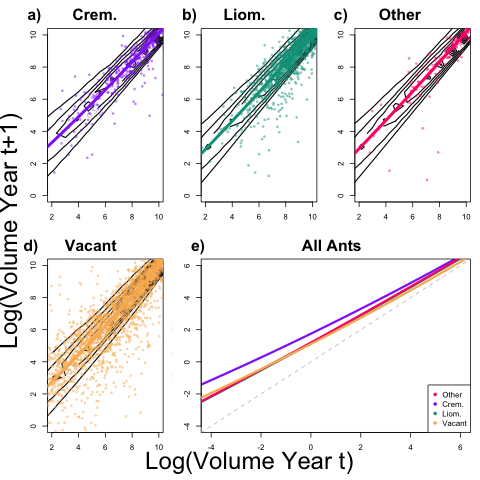
\includegraphics[width = 0.95\linewidth]{Figures/GrowContourLinesColor.png}
	\caption{This figure shows the next predicted size of cholla based on previous size with each individual ant partner. The solid colored lines (seen in all panels) are the next mean predicted size of cholla. The points (seen in panels a-d) are the observed data which informs these estimates. The black countour lines (seen in a-d) appear at 5\% increments showing where 5\%, 10\%, etc. of the data is expected to fall. They grey dashed line (in panel e only) shows the line where the next predicted size is the same as the previous (aka there is no growth on this line and below this line is shrinkage). }
	\label{fig:Grow}
\end{figure}

\paragraph{Survival Model}
We found evidence that ant visitation enhances the survival of medium to large plants, and that partner identity has a significant impact on survival for smaller plants (Figure \ref{fig:Surv}).
Tree cholla experience between 7.7\% and 99.9\% survival rates depending on 
their size and ant partner (Figure \ref{fig:Surv}e).
Smaller cacti all have lower survival rates, while larger cacti have higher survival rates, all nearing 100\% when they reach their largest observed sizes.
Plants with \textit{C. opuntiae} ants experience the highest mean survival rates across all sizes (Figure \ref{fig:Surv}a).
Plants with \textit{L. apiculatum} ants experience the lowest mean survival rates when small and the second highest mean survival rates across all other sizes (Figure \ref{fig:Surv}b). 
Plants with other ants experience the second lowest mean survival rates across all sizes (Figure \ref{fig:Surv}c).
Plants with no partners experience the second highest survival rates at small sizes, after which they experience the lowest survival rates (Figure \ref{fig:Surv}d). 

Using the method of subtracting one survival distribution from another we were able to determine how confident we are that the survival of cholla visited by one combination of ant partners is more likely than another. 
$S_{Crematogaster} - S_{Vacant}$ returns a vector which is 82\% positive, meaning we are 82\% confident that when \textit{C. opuntiae} ants are partners the survival of the cholla is more likely than the survival of the cholla with no ant partners.
Given the evidence that plants visited by \textit{C. opuntiae} experience the highest mean survival rates we have reported our confidence that this partner is associated with the highest survival rates below. 
We are 63\% and 100\% confident that plants tended by \textit{C. opuntiae} ants experience higher mean survival rates across all sizes than plants tended by \textit{L. spiculatum} ants or other ants respectively.
We are 82\%, 68\%, and 64\% confident that plants with no partners experience lower mean survival rates across all sizes than plants tended by 

\begin{figure}[H]
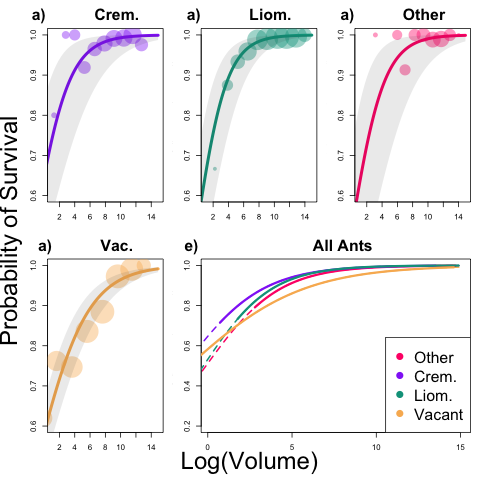
\includegraphics[width=0.95\linewidth]{Figures/SurvivalPlot.png}
\caption{This figure shows the estimated survival rates based on the size of the cactus with each individual ant partner. The solid colored lines (shown on all panels) indicate the mean estimated survival rates. The dashed lines (shown in panel e) indicate extrapolations beyond existing data (where we estimated survival for plants tended by ants where we had never seen a tended cactus of that size). The grey area around the solid lines (shown in panels a-d) show the 90\% confidence interval for the estimates. The colored dots are the real data binned by size to show how our estimates align with real survival observations. A larger circle means we had more data on survival of plants of this size with this partner.}
\label{fig:Surv}
\end{figure}

\paragraph{Viability Model}
We found evidence that ant visitation leads to increased floral viability rates and that ant identity can influence the strength of viability.
Tree cholla that are reproducing in year $t$ experience between 39\% and 96\% viability rates of flowers (Figure \ref{fig:viab}).
The ant partners make a difference in the mean viability rate of flowers, with \textit{L. apiculatum} tended plants experiencing the highest mean viability rate (at 86\%, Figure \ref{fig:Viab}b), followed by other tended plants (at 75\%, Figure \ref{fig:Viab}c), \textit{C. opuntiae} tended plants (at 74\%, Figure \ref{fig:Viab}a) and vacant plants (at 71\%, Figure \ref{fig:Viab}d).

Using the method of subtracting one viability distribution from another we were able to determine how confident we are that the floral viability of cholla visited by one combination of ant partners is greater than another. 
$V_{Liomatopum} - V_{Vacant}$ returns a vector which is 99\% positive, meaning we are 99\% confident that when \textit{L. apiculatum} ants are partners the floral viability of the cholla is greater than the cholla with no ant partners.
Given the evidence that plants visited by \textit{L. apiculatum} experience the highest viability rates we have reported our confidence that this partner is associated with the highest viability rates below. 
We are 98\% and 97\% confident that \textit{L. apiculatum} tended plants experience higher viability rates than plants tended by \textit{C. opuntiae} or other ants respectively.
We are 95\% and 69\% confident that vacant plants experience lower viability rates than plants tended by \textit{C. opuntiae} ants or other ants respectively.

\begin{figure}[H]
	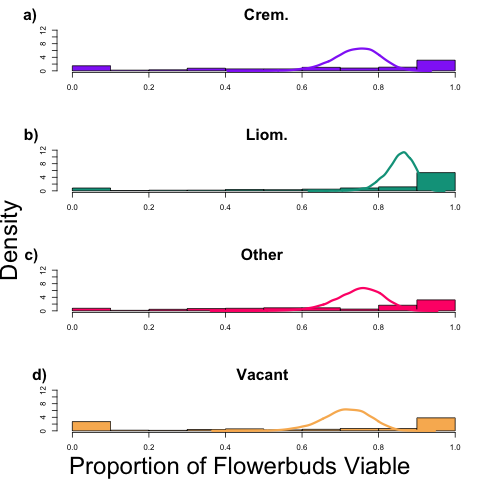
\includegraphics[width=0.95\linewidth]{Figures/ViabHist.png}
	\caption{This figure shows the estimated distributions of floral viability rates compared to observed distributions of floral viability rates of cholla based on ant partner identity. The solid lines indicate the estimated viability distribution. The colored histograms represent the observed viability rates of plants with that partner. }
	\label{fig:Viab}
\end{figure}

\ali{}{Should I include other model results here or just indicate that the rest are reported in an appendix/supplementary materials?}

\subsubsection*{The role of annual fluctuations in demographic effects of ant partners}
We found evidence that annual variation impacts the effect of ant partner on various demographic traits (Figure \ref{fig:Annual_Ant}).
The effects of each partner on demographic measure vary uniquely across temporal fluctuations, making partner identity important to track in conjunction with annual variation. 
Specifically, where some ants offered greater than average benefits in one year, other species offered reduced benefits in the same year, indicating that each ant partner reacts differently to the fluctuating environment. 

Each demographic trait was not affected equally by the intersection of ant partner and annual fluctuations.
We looked at the mean effect of each ant partner on growth (figure \ref{fig:Annual_Ant}a), survival (Figure \ref{fig:Annual_Ant}b), and viability (Figure \ref{fig:Annual_Ant}c) rates across all the years included in our study. 
Where the mean effect is exactly 0 there is missing ant data due to variation in censusing focus.
This is an indirect way to analyze how temporal fluctuation impacts our system without attributing the effects to a specific climate variables. 
Where the mean effect is positive, ant presence increases the respective estimated growth, survival, or viability rates in response to environmental fluctuations, and where the mean effect is negative, the opposite occurs. 
We found the general magnitude of variation was the smallest for the growth rate, meaning annual variation affected the growth of plants the least, followed by survival then viability. 

\begin{figure}[H]
	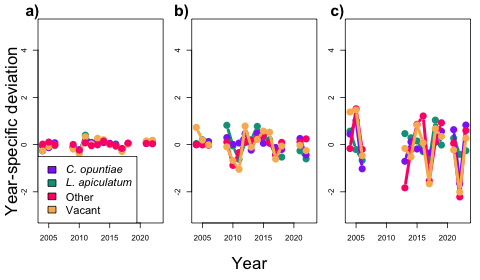
\includegraphics[width=0.95\linewidth]{Figures/year_ant_timeseries.png}
	\caption{This figure shows the mean affect of each ant partner on a) the estimated next size, b) the estimated survival, and c) the floral viability of cacti across every year of our study. These values are estimated from the fitted random effects of ant and year in our models. Each point represents the mean of the random effect of the identified model, ant, and year (e.g. the lowest dot in panel b) represents the mean effect of vacancy on survival rates in year 2011).}
	\label{fig:Annual_Ant}
\end{figure}

\subsection*{What are the frequency and direction of partner turnover across the plant life cycle?}
We found that there is a high frequency of partner turnover observed in this system with very distinct directional patterns. 
Small plants are almost always vacant (Figure \ref{fig:Ant_Transition}b-d), if they were previously tended by a partner, they are likely to become vacant again (Figure \ref{fig:Ant_Transition}a).
As the size of the plants increases, the probability of becoming tended increases as well, though it is not equally likely to be tended by all partners. 

\textit{L. apiculatum} ants become the most likely next partner in the case of most large plants, with the exception of a large plant which was previously tended by \textit{C. opuntiae}.
Plants which were previously tended by \textit{C. opuntiae} ants are most likely to remain tended by \textit{C. opuntiae} ants.
This indicates that these species may follow the well documented retention-discovery trade off exhibited  by many ants, with \textit{L. apiculatum} ants excelling at discovery and colonization of new plants and \textit{C. opuntiae} ants excelling at plant retention season after season.
The overall frequency of these partners, however is a potential alternative explanation to this discovery-retention trade off.
\textit{L. apiculatum} ants are by far the most frequent ant partners, accounting for 75\% of the occupied cacti, while \textit{C. opuntiae} and other ants account for 17\% and 8\% of occupied cacti respectively.
This high frequency of \textit{L. apiculatum} ants may lead to the inflation of turnover to \textit{L. apiculatum} from other ants. 

\begin{figure}[H]
	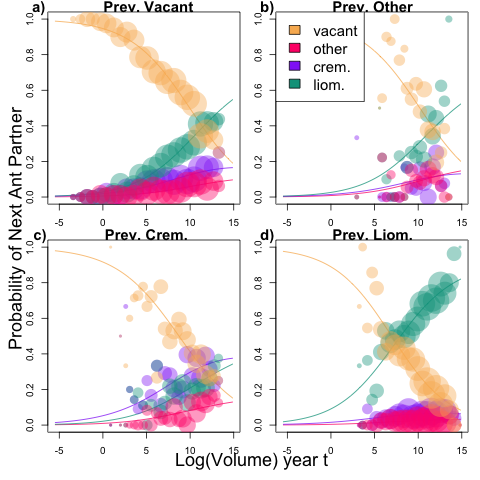
\includegraphics[width=0.95\linewidth]{Figures/AntSizeMulti.png}
	\caption{This figure shows the probability of being tended by each ant partner or vacant based on the size of the plant. Each panel shows these probabilities for a different previous ant state. The solid lines represent the mean probability of being tended by a specific partner. The colored points are the real data binned by size to show how our estimates align with real visitation observations. A larger circle means we had more data on visitation of plants of this size with this previous partner.}
	\label{fig:Ant_Transition}
\end{figure}

\subsection*{What is the net effect of partner diversity on plant fitness, and what mechanism(s) explain(s) this effect?}
We found that partner diversity was beneficial in this system. 
The lowest mean fitness was $\lambda_{S,Vacant}$, the fitness of the cholla with no partners (Figure \ref{fig:LambdaMeans}b).
By subtracting the distributions $\lambda_{S, any} - \lambda_{S,Vacant}$, we found that we are between 82\% and 100\% confident that having any partner leads to a higher population fitness than having no partner. 
If you consider just the number of partners (ignoring the identity), what you find is actually that the more partners are present, the higher the fitness of the cacti (Figure \ref{fig:LambdaMeans}b), though this increase is primarily driven by the presence of \textit{L. apiculatum}.

\begin{figure}
	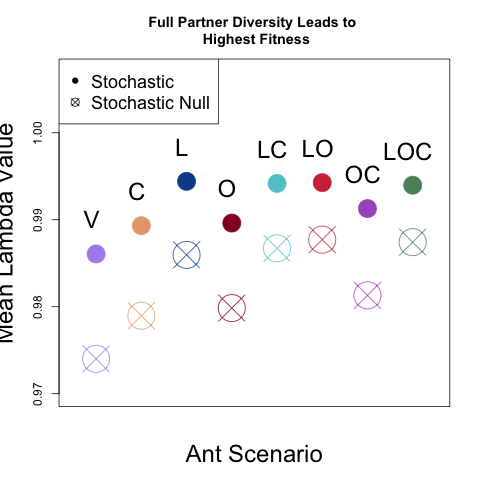
\includegraphics[width=0.61\linewidth]{Figures/LambdaMeans.png}
	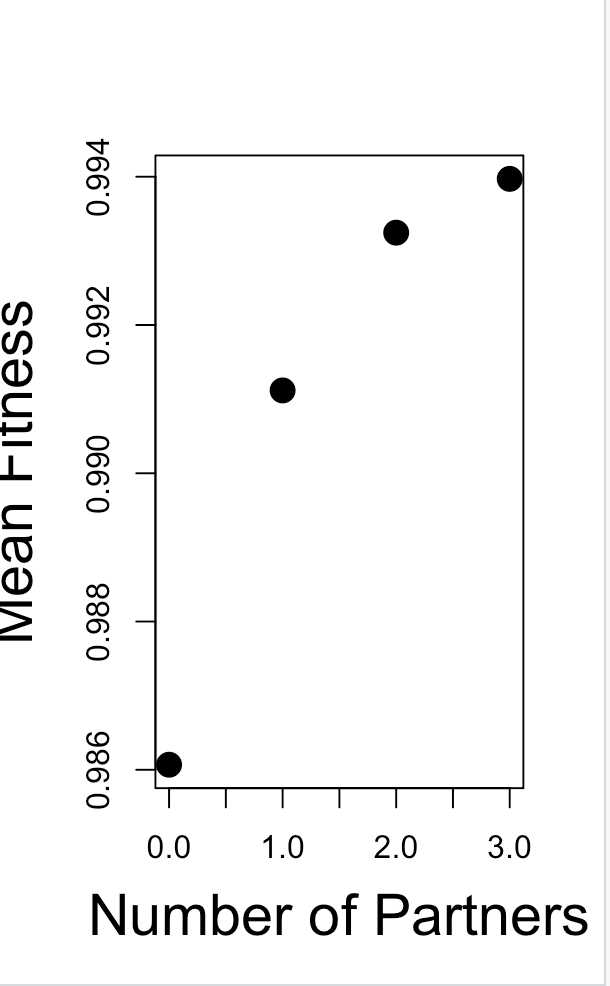
\includegraphics[width=0.39\linewidth]{Figures/Lambda_Num_Partners.png}
	\caption{Panel a) shows the mean values of the estimated $\lambda_{S}$ (filled in circles) and $\lambda_{SN}$ (empty circles with an X) for each simulated combination of ant partners. The letters above the points correspond to what ant partners are present (V = Vacant, C = \textit{C. opuntiae}, L = \textit{L. apiculatum}, O = other). Panel b) shows the mean values of the estimated $\lambda_{S}$ for }
	\label{fig:LambdaMeans}
\end{figure}

Despite this apparent synergy, when partner identity was considered, we found the benefits of partner diversity could be explained by Sampling Effect.
We believe the benefits of partner diversity are heavily driven by the presence of a single best partner rather than overall synergy.
All simulated combinations of ant partners which included \textit{L. apiculatum} were nearly equal and the highest possible fitness estimated for the cholla. 
This indicates that \textit{L. apiculatum} are the single best partner for the cholla under existing conditions. 
Based on the definitions of Sampling Effect and Complementarity we use in this study \citep{Batstone2018}, it is clear that Sampling Effect can explain the benefits of partner diversity in the cholla system. 

It is possible that this, like the frequency of partner turnover to \textit{L. apiculatum}, is driven by the extreme frequency of \textit{L. apiculatum} ants in comparison to others. 
With this in mind, we simulated the population fitness with equal probability for transitioning to any ant state.
We found ...... from the simulations with different transition probabilities.
 \ali{}{This feels like the most natural progression to me.}

We found evidence of portfolio effect, meaning the presence of multiple partners did not buffer against the potentially negative effects of annual fluctuations.
The effect of all ant partners can be measured as $\lambda_{All} - \lambda_{Vacant}$ (Figure \ref{fig:Portfolio}).
We are are 94\% confident that when all ants are present the cholla experience higher fitness than when no ants are present according to both the stochastic and stochastic null model. 
When subtracting these two resulting vectors from each other (($\lambda_{S,All} - \lambda_{S,Vacant}$) - ($\lambda_{SN,All} - \lambda_{SN,Vacant}$)), we found that we are only 52\% confident that partners offer higher benefits when able to respond uniquely to a fluctuating environment. 
\ali{There is no real difference between the two scenarios, meaning we have no evidence of portfolio effect.}{I am not sure if I have explained enough here honestly.}

\begin{figure}
	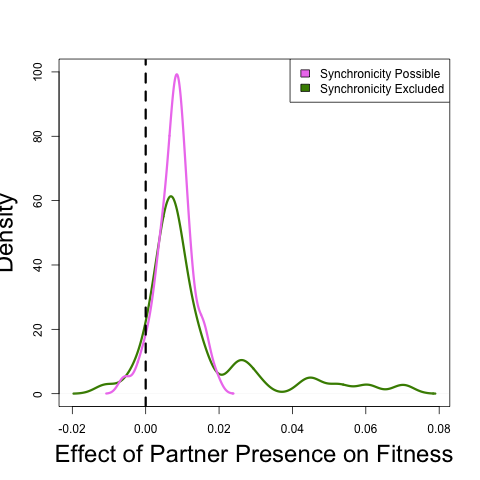
\includegraphics[width=\linewidth]{Figures/portfolio_effect.png}
	\caption{This figure shows the distribution of $\lambda_{S,All}-\lambda_{S,Vacant}$ in pink and $\lambda_{SN,All}-\lambda_{SN,Vacant}$ in green. The vertical dashed line shows where the effect of partners on the fitness of the cholla is 0 (to the left the partners have a negative effect, to the right the partners are beneficial).}
	\label{fig:Portfolio}
\end{figure}

\section*{Discussion}
\tom{}{I have not commented too heavily here because I would like to talk through what we want this section to achieve. Currently, most of this section is actually describing results, whereas the pupose is to interpret and contextualize results, and connect them to the broader literature. Some of your content here is actually better at describing results than you had in the Results section, because it includes that element of ``how is this connected to the question'' that was missing from the Results section.}
The large, long-lived tree cholla produce EFN which tempts several species of ant partners to protect them from herbivores and seed predators. 
Many studies have looked at multispecies mutualisms and the how having a variety of partners leads to variation in demographic effects \cite{Palmer2010, Bascompte2019, Stachowicz2005, Ford2015, Baez2016}. 
Because these tree cholla interact with only one ant partner at a time, it is a unique system in which to parse out the individual effects of each ant partners, both in isolated settings or in combinations we cannot test in the real world. \tom{}{This is a good start. In general, I suggest opening the Discussion section with a brief summary of what you were trying to learn in this study, what you found, and its broader significance. This paragraph does a little of that, but I think it can be stronger.}


%\subsection*{Demographic effects of association with alternative partners}
We asked what effects the partners which interact with tree cholla (\textit{C. opuntiae},\textit{L. apiculatum}, \tom{and more}{I would not say this.}) have on the vital rates of tree cholla. 
Using a system of heirarchical bayesian models we found that there were discernable differences in the effects that each partner had on vital processes of the focal mutualist. 
The different vital rates vary in importance across tree cholla ontogeny.
Several of them are negatively impacted by the presence and pressure of herbivores and seed predators \cite{Miller2009, Miller2006} and positively impacted by the presence of ant partners \cite{Miller2007}.
The predators and herbivores target new growth and flowers, leading to negative impacts on the growth rates, survival rates, and floral viability rates of tree cholla \cite{Louda1995, Agrawal2004}.
The presence of the ant partners can reduce those negative effects.


It has been previously hypothesized that their is a heirarchy of partners due to the ability for \textit{L. apiculatum} ants to defend the cacti from seed predators and herbivores \cite{Miller2007}.
These prior results would suggest that all vital rates that are affected by ant partners would be boosted the most by the presence of \textit{L. apiculatum} ants, this is not what we found. 
Our results suggest that different partners differ significantly in their effects on vital rates.

Prior to reproduction, the tree cholla experience only growth and survival.
\textit{C. opuntiae} tended ants are associated with the highest growth rates and survival rates of plants. 
This indicates that \textit{C. opuntiae} ants may be good ants for pre-reproductive tree cholla plants. 
Reproducing plants experience a probability of reproducing, flower production, and floral abortion.
\tom{Floral abortion is heavily affected by seed predators \cite{Miller2008}}{Seed predators do not influence floral abortion.}, which the ants defend the cacti, leading to increased floral viability.
We specifically found that tree cholla experienced the highest floral viability rates when tended by \textit{L. apiculatum} ants. 
This indicates that \textit{L. apiculatum} ants may be good partners for reproducing plants. 

These results together would suggest that complementarity may be the underlying mechanism that explains why partner diversity is beneficial in this system. 


%\subsection*{Frequency and direction of partner turnover}
We have shown that the identity of partners is important to the processes that define tree cholla fitness. 
Now we need to analyze the dynamics of partner turnover which dictate the identity of tree cholla partners and therefore the effects of vital rates on the tree cholla. 
With our models we were able to identify both the direction, frequency, and distinct patterns of partner turnover. 

In the literature, it is clear that the frequency of partner turnover can have big effects on the fitness of the focal mutualist \cite{Fiala1994, Horvitz1986, Oliveira1999, Sachs2004}.
In some systems high freqency of turnover is necessary to resiliency and leads to higher fitness benefits \cite{Trojelsgaard2015}, while in other systems loyalty is the most beneficial \cite{Batstone2018}.
While the purpose of this paper is not to establish which would be most beneficial in this system, we were able to identify the pattern. 
Small plants are almost entirely vacant in this system until they grow large enough to begin producing significant amounts of EFN.
Our model shows that once they do produce EFN, plants experience a relatively significant amount of turnover.
Mid-sized and large plants which were either vacant or tended by other ants are most likely to become tended by \textit{L. apiculatum} ants in the next year, thereby experiencing partner turnover. 
Plants which were tended by \textit{L. apiculatum} or \textit{C. opuntiae} ants are most likely to remain tended by the same partners multiple years in a row. 
This indicates that \textit{C. opuntiae} ants and \textit{L. apiculatum} ants are loyal partners which retain the same plants year after year with regularity.


As established in previous studies, the direction of partner turnover is important when the identity of partners impacts the quality of benefits recieved \cite{Fonseca2003, Alonso1998, Dejean2008, Noe1994}.
In our study we found that there are distinct patterns to the direction of partner turnover. 
Specifically, most plants are tended by \textit{L. apiculatum} ants at some point, because vacant plants, other tended plants, and \textit{L. apiculatum} tended plants are all most likely to be tended by \textit{L. apiculatum} ants.
This indicates that while \textit{L. apiculatum} ants are loyal to their own plants and return multiple years in a row to the same ones, they are also strong colonizers. 


%\subsection*{Effect of partner diversity on plant fitness and what mechanisms explain this}
The combination of partner identity, partner turnover, and temporal stochasticity gives us the unique power to consider both the fitness of the tree cholla under different partner scenarios (\tom{as some have done before \cite{Palmer2010}}{There is more than just the Palmer pape. Be sure that you are comprehensive in your use of the literaure, include non-ant-plant studies,}) and a unique set of mechanisms (\cite{Batstone2018}) which explain how the multi-partner interactions lead to fitness differences. 
We found that the combination of \tom{accurate partner transitions with partner identity}{Not sure what this means.} affected the fitness of the tree cholla in interesting and dynamic ways. 
Namely, a best partner emerged in this analysis, which was surprising given the nature of our vital rate findings. 
The variation in best partner for each vital rate suggested the potential that the different ant partners had some level of unique specialty in what they offered, which would support complementarity as the mechanism which explained the effects of partner diveristy \cite{Stachowicz2005, Stanton2003}. 
The results of our IPM however differ from this prediction. 

Using the stochastic IPM we developed, we found evidence of sampling effect rather than complementarity.
We found that \textit{L. apiculatum} was the single best partner, and that all diversity scenarios where \textit{L. apiculatum} was present resulted in the highest possible fitness of tree cholla. 
This indicates that despite the fact that \textit{L. apiculatum} partnership does not result in the highest growth and survival rates, it is still the overall best partner. 

Using the stochastic null IPM and the stochastic IPM we compared the fitness boost recieved by all ant partners when ants effects varied separately across years and when they did not. 
When all ants responded to inter-annual variability the same way (shown in the stochastic null IPM) we found that the fitness boost recieved from partners was larger than the fitness boost recieved when ants responded to inter-annual variability differently.
This indicates that having multiple possible partners benefits the tree cholla by buffering the potentially negative effects of inter-annual variation. 

%\subsection*{Synthesis????? All together}
\ali{}{What this all means more broadly?? I'm currently not sure what to do with this. Tom: that's the entire Discussion!}
This paper shows the importance of long-term datasets in investigating species interactions and calls for further use of long-term data. 
\tom{Previously studies have analyzed how partner identity and partner turnover impact focal mutualist fitness \cite{Fonseca2003, Dejean2008, Noe1994, Barrett2015, Bruna2014, Trojelsgaard2015}.
Separate studies have analyzed how inter-annual variability impacts focal mutualists \cite{Alonso1998, Alarcon2008, Ollerton2006, Horvitz1990, Lazaro2022}.
The long term dataset we used gave us the unique ability to consider the combined effects of partner identity, partner turnover, and temporal stochasticity.}{This is really good. More of this!}


%\subsection*{Future Directions}
\tom{This paper has limitations, specifically surrounding the driving forces behind the ant-plant interactions.
We revealed the dynamics of partner turnover and showed that different ant partners are correlated with different fitness benefits.
As of now, the driving mechanisms behind how ant species come to interact with individual plants is still unknown and could be subject to future work. }{This feels a little weak and incomplete.}


\section*{Acknowledgments}
This should be drafted.
%%%%%%%%%%%%%%%%%%%%%
% Statement of Authorship
%%%%%%%%%%%%%%%%%%%%%
% This section should also be commented out while your MS is undergoing
% double-blind review. The specifics should of course be adapted to
% your paper, but the paragraph below gives some hints of possible
% contributions.

\section*{Data and Code Availability}
This should be drafted.

\section*{Appendix A: Additional Methods and Parameters}
This is not referenced in the paper, to my knowledge, and I think you need to think more deeply about what content should go into appendices and why. 
% In most cases, authors should typeset supplementary material in a separate,
% author-supplied PDF. For author-supplied PDFs, please consult the
% AmNat_supp_template.tex document, available from
% https://www.journals.uchicago.edu/journals/an/instruct 
%
% By contrast, the Appendix instructions below apply to cases in which
% a brief appendix is to appear in print after the main body of the article.
% That notably includes descriptions of methods, tables defining parameters,
% and other material necessary for reproducing the MS's results.
%
% Please reset counters for the appendix (thus normally figure A1, 
% figure A2, table A1, etc.).
%
% Most AmNat articles have no more than one print appendix. If your article
% has more than one, counters for each appendix should match the letter of
% that appendix. For example, tables in Appendix B should be numbered table B1, % table C2, etc. This applies to tables, equations, and figures.
%
% It's better not to use the \appendix command, because we have some
% formatting peculiarities that \appendix conflicts with.

\renewcommand{\theequation}{A\arabic{equation}}
% redefine the command that creates the equation number.
\renewcommand{\thetable}{A\arabic{table}}
\setcounter{equation}{0}  % reset counter 
\setcounter{figure}{0}
\setcounter{table}{0}

%%%%%%%%%%%%%%%%%%%%%
% Bibliography
%%%%%%%%%%%%%%%%%%%%%
% You can either type your references following the examples below, or
% compile your BiBTeX database and paste the contents of your .bbl file
% here. The amnatnat.bst style file should work for this---but please
% let us know if you run into any hitches with it!
%
% If you upload a .bib file with your submission, please upload the .bbl
% file as well; this will be required for typesetting.
%
% The list below includes sample journal articles, book chapters, and
% Dryad references.
\bibliographystyle{apalike}
\bibliography{References.bib}


\newpage{}

\section*{Tables}
\renewcommand{\thetable}{\arabic{table}}
\setcounter{table}{0}

\renewcommand{\thetable}{\arabic{table}}
\setcounter{table}{0}

% I am creating a table here to include all parameter estimations and descriptions
  \begin{table}[]
  \begin{tabular}{l|l|l}
    \textbf{Parameter} & \textbf{Median ($95\%$ CI)} & \textbf{Prior Distribution} \\
    \hline
    %% Growth Parameters
    growth xi intercept vacant $\beta_{01}^g$ & $-5.210899 (-5.686865, -5.491787)$ & sDE\\
    growth xi intercept other $\beta_{02}^g$ & $-5.8288 (-5.956217, 1.766021) $&asdf \\
    growth xi intercept \textit{C. opuntiae} $\beta_{03}^g$ & $-4.529523 (-6.0770390, 0.1222112)$ & asdf\\
    growth xi intercept \textit{L. apiculatum} $\beta_{04}^g$ & $-5.106802 (-5.4499944, 0.5453901)$ & asdf\\
    growth xi size dependent vacant $\beta_{11}^g$ & asdf&asdf \\
    growth xi size dependent other $\beta_{12}^g$ & asdf&asdf \\
    growth xi size dependent \textit{C. opuntiae} $\beta_{13}^g$ & asdf&asdf \\
    growth xi size dependent \textit{L. apiculatum} $\beta_{14}^g$ &sadf &asdf \\
    growth omega intercept $\omega_0^g$ & & \\
    growth omega size dependent $\omega_1^g$ & & \\
    growth alpha intercept $\alpha_0^g$ & & \\
    growth alpha size dependent $\alpha_1^g$ & & \\
    \hline
    %% Germination Parameters
    1-year germination intercept $\alpha^{\gamma_1}$ & & \\
    2-year germination intercept $\alpha^{\gamma_2}$ & & \\
    \hline
    %% Survival Parameters
    survival intercept vacant $\beta_{01}^s$ & & \\
    survival intercept other $\beta_{02}^s$ & & \\
    survival intercept \textit{C.opuntiae} $\beta_{03}^s$ & & \\
    survival intercept \textit{L. apiculatum} $\beta_{04}^s$ & & \\
    survival size dependent vacant $\beta_{11}^s$ & & \\
    survival size dependent other $\beta_{12}^s$ & & \\
    survival size dependent \textit{C. opuntiae} $\beta_{13}^s$ & & \\
    survival size dependent \textit{L. apiculatum} $\beta_{14}^s$ & & \\
    \hline
    %% Probability of Flowering Parameters
    flowering intercept $\beta_0^f$ & & \\
    flowering size dependent $\beta_1^f$ & & \\
    \hline
    %% Floral Viability Parameters
    viability intercept vacant $\beta_01^v$ & & \\
    viability intercept other $\beta02^v$ & & \\
    viability intercept \textit{C. opuntiae} $\beta_03^v$ & & \\
    viability intercept \textit{L. apiculatum} $\beta_04^v$ & & 

  \end{tabular}
  \caption{This table includes the median estimates, the 95$\%$ confidence intervals, and the prior distribution for each parameter in each model.}
  \label{tab:Params}
  \end{table}

\section*{Figure legends}

\section*{Supplementary Materials}
\subsection*{Herbivory Data}
\subsection*{Model Checks}
For each model fitted, we conducted two tests to determing if the fit was acceptable to use in our IPM. 
First, we checked the convergence of each parameter.
Below we show the convergence of all $\beta$ terms listed in the Statistical Modeling subsection of Methods.
Second, we checked the posterior fit, comparing the estimated values of each model to the $y$ values of the actual data.
We show these posterior checks below, split by ant partner where relevant.
%% Growth Figure
%% Survival Figure
\begin{figure}
	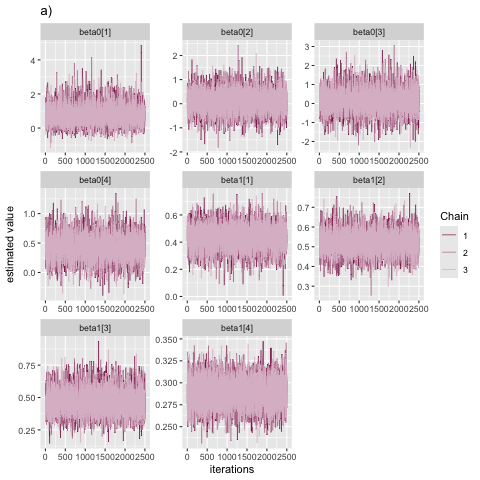
\includegraphics[width = 0.45\linewidth]{Figures/surv_conv.png}
	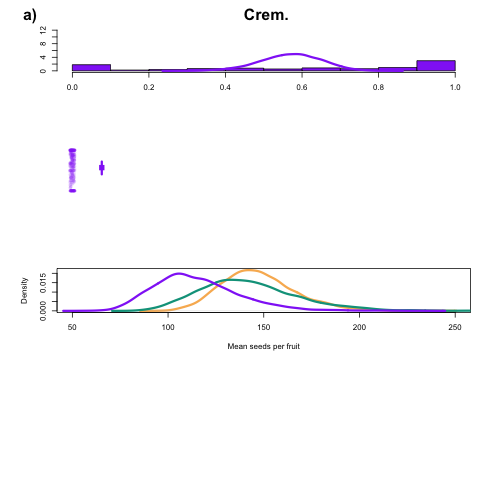
\includegraphics[width=0.45\linewidth]{Figures/surv_post.png}
	\caption{The a) posterior convergence of the parameters estimated by the survival model and the b) posterior distribution of survival estimates (pink lines) for each ant species (1 = \textit{C. opuntiae}, 2 = \textit{L. apiculatum}, 3 = other, 4 = vacant) compared to the mean survival distribution (black line) of the real data.}
	\label{fig:Surv_post}
\end{figure}
%% Reproduction Figure
\begin{figure}
	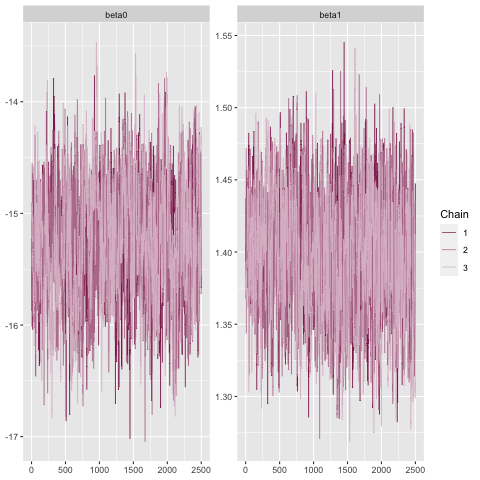
\includegraphics[width = 0.45\linewidth]{Figures/repro_conv.png}
	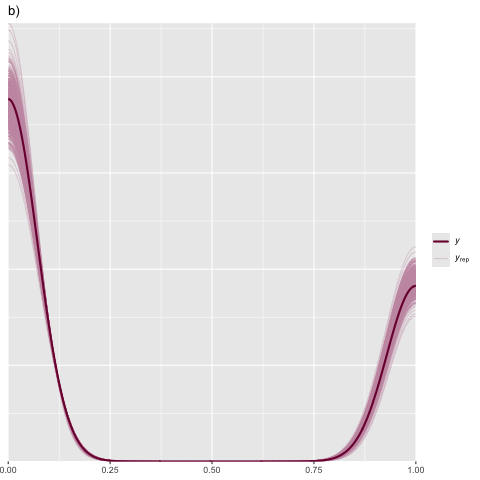
\includegraphics[width=0.45\linewidth]{Figures/repro_post.png}
	\caption{The a) posterior convergence of the parameters estimated by the reproduction model and the b) posterior distribution of reproductive status estimates (pink lines) for each ant species (1 = \textit{C. opuntiae}, 2 = \textit{L. apiculatum}, 3 = other, 4 = vacant) compared to the mean reproductive status distribution (black line) of the real data.}
	\label{fig:Repro_post}
\end{figure}
%% Flowering Figure
\begin{figure}
	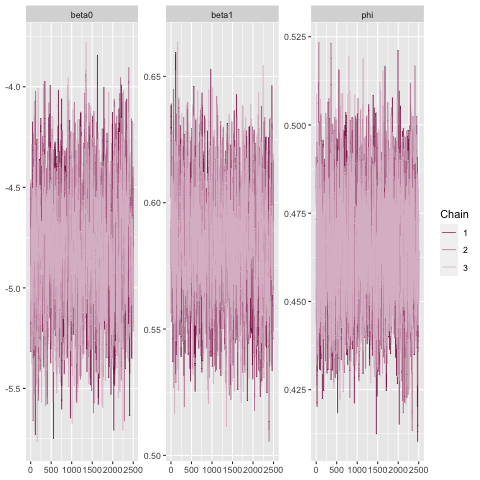
\includegraphics[width = 0.45\linewidth]{Figures/flow_conv.png}
	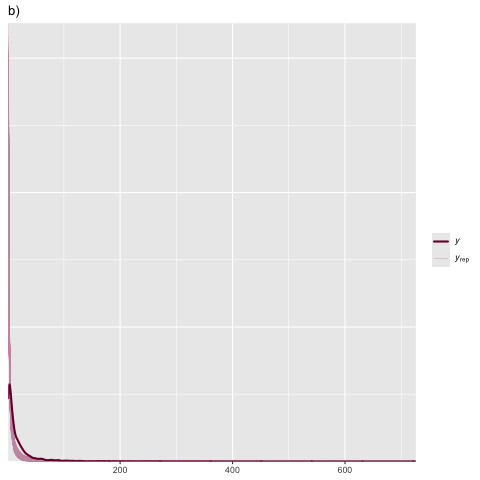
\includegraphics[width=0.45\linewidth]{Figures/flow_post.png}
	\caption{The a) posterior convergence of the parameters estimated by the number of flowers model and the b) posterior distribution of the number of flowers estimated (pink lines) compared to the mean distribution of observed flowers (black line).}
	\label{fig:Flow_post}
\end{figure}
%% Viability Figure
\begin{figure}
	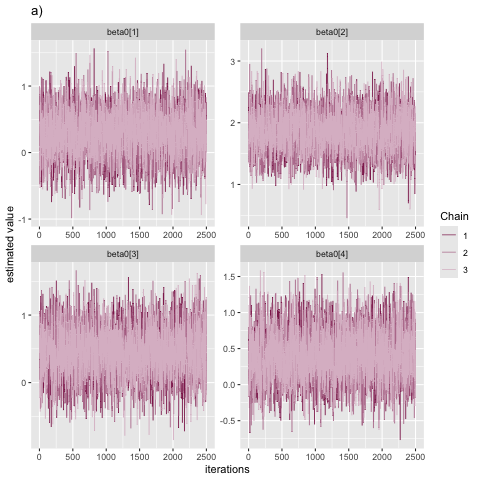
\includegraphics[width = 0.45\linewidth]{Figures/viab_conv.png}
	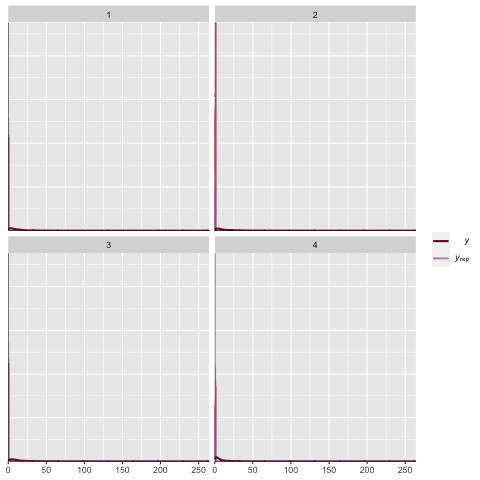
\includegraphics[width=0.45\linewidth]{Figures/viab_post.png}
	\caption{The a) posterior convergence of the parameters estimated by the viability model and the b) posterior distributions of floral viability estimates (pink lines) for each ant species (1 = \textit{C. opuntiae}, 2 = \textit{L. apiculatum}, 3 = other, 4 = vacant) compared to the mean floral viability distribution (black line) of the real data.}
	\label{fig:Viab_post}
\end{figure}
 %% Seeds Per Fruit
 \begin{figure}
 	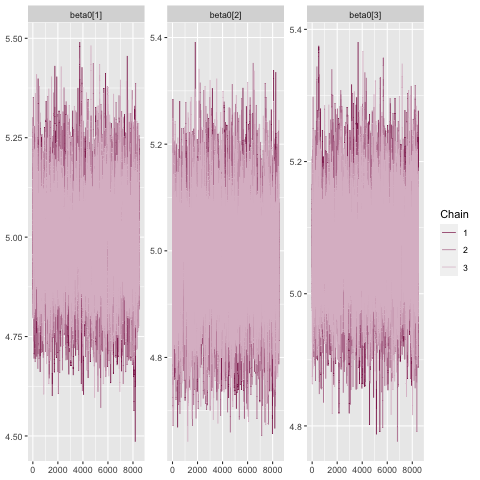
\includegraphics[width = 0.45\linewidth]{Figures/seed_conv.png}
 	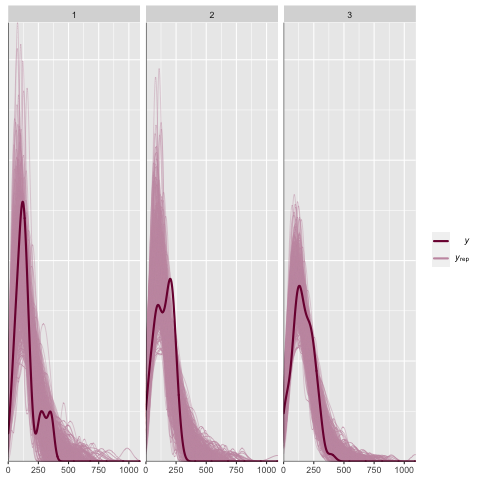
\includegraphics[width=0.45\linewidth]{Figures/seed_ant_post.png}
 	\caption{The a) posterior convergence of the parameters estimated by the seeds per fruit model and the b) posterior distributions of seeds per fruit estimates (pink lines) for each ant species (1 = \textit{C. opuntiae}, 2 = \textit{L. apiculatum}, 3 = vacant) compared to the mean seeds per fruit distribution (black line) of the real data.}
 	\label{fig:seed_post}
 \end{figure}
 %% Fruit survival 
% \begin{figure}
%% 	\includegraphics[width = 0.45\linewidth]{Figures/                .png}
%% 	\includegraphics[width=0.45\linewidth]{Figures/               .png}
% 	\caption{The a) posterior convergence of the parameters estimated by the fruit survival model and the b) posterior distributions of fruit survival estimates (pink lines) compared to the mean fruit survival distribution (black line) of the real data.}
% 	\label{fig:fruit_surv_post}
% \end{figure}
% %% Ant Transitions
% \begin{figure}
%% 	\includegraphics[width = 0.45\linewidth]{Figures/             .png}
%% 	\includegraphics[width=0.45\linewidth]{Figures/               .png}
% 	\caption{The a) posterior convergence of the parameters estimated by the ant transitions model and the b) posterior distributions of next ant partners estimates (pink lines) for each previous ant species (1 = \textit{C. opuntiae}, 2 = \textit{L. apiculatum}, 3 = other, 4 = vacant) compared to the mean next ant partner distribution (black line) of the real data.}
% 	\label{fig:Transitions_post}
% %% Germination
 \begin{figure}
 	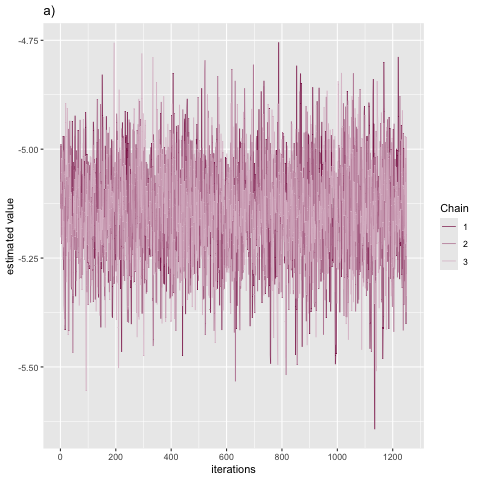
\includegraphics[width = 0.45\linewidth]{Figures/germ1_conv.png}
 	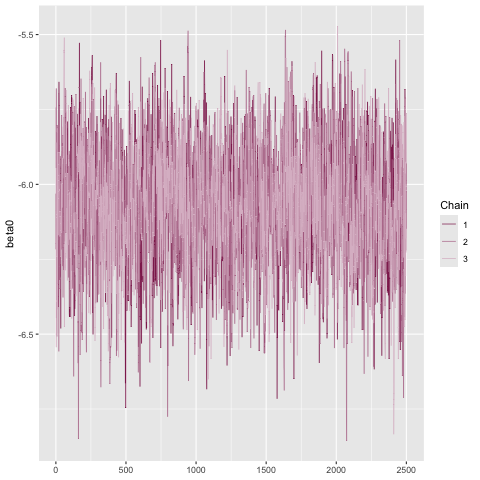
\includegraphics[width=0.45\linewidth]{Figures/germ2_conv.png}\\
 	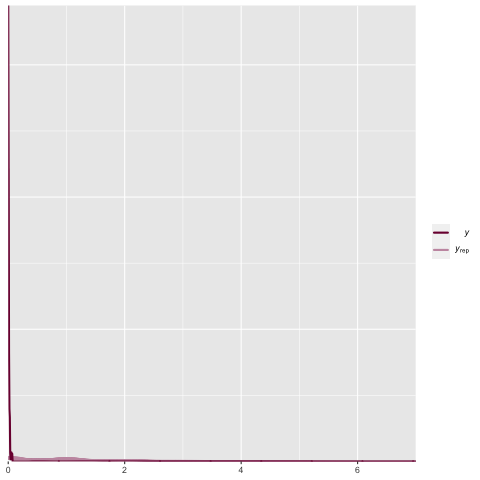
\includegraphics[width=0.45\linewidth]{Figures/germ1_post.png} 	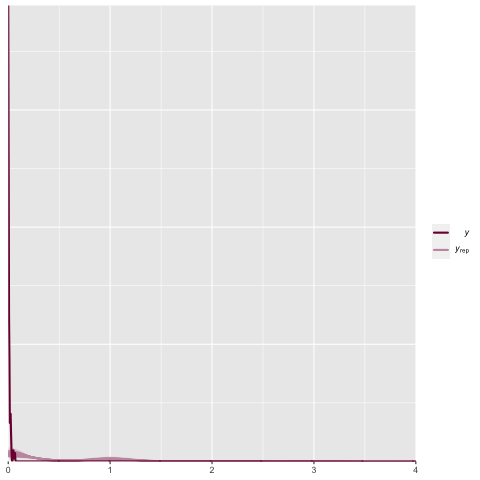
\includegraphics[width=0.45\linewidth]{Figures/germ2_post.png}
 \caption{The a-b) posterior convergence of the parameters estimated by the germination from year one seedbank and germination from year two seedbank models respectively. The c-d) posterior distributions of floral viability estimates (pink lines) compared to the mean germination distribution (black line) of the real data for first year germinants and second year germinants respectively.}
 	\label{fig:Germ_post}
 \end{figure}

 %% Pre-Census Survival
 \begin{figure}
 	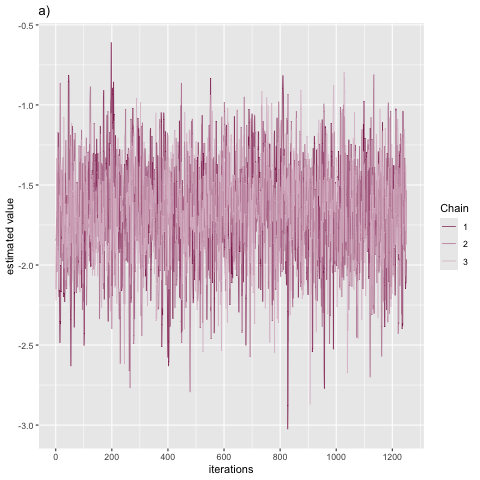
\includegraphics[width = 0.45\linewidth]{Figures/seed_surv_conv.png}
 	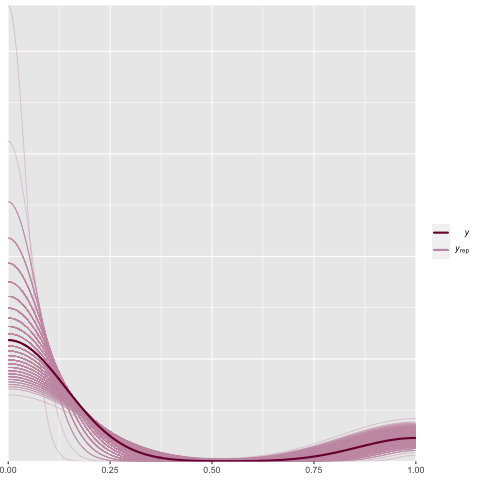
\includegraphics[width=0.45\linewidth]{Figures/seed_surv_post.png}
 	\caption{The a) posterior convergence of the parameters estimated by the pre-census survival model and the b) posterior distribution of the pre-census survival estimated (pink lines) compared to the mean distribution of observed pre-census survival (black line).}
 	\label{fig:Pre_Surv_post}
 \end{figure}
 %%
 
 \subsection*{Statistical Models -- Results}
 Below are the results reorted of all statistical models not described in the main body of the text. 
 
 %% Reproduction Model
 \paragraph{Reproduction Model}
 The probability of a plant reproducing in a given year is highly size dependent. 
 The mean probability of reproducing remains at about 0\% until the plant reaches a medium size, after which the mean probability of reproducing increases steadily before reaching about 100\% at large sizes. 
 
 
 
 %% Seeds Produced
 \paragraph{Seeds Per Flower Model}
 Each viable flower on a plant produces between 97 and 257 seeds.
 \tom{This number is affected by the ant partner present. 
 	\textit{C. opuntiae} tended plants produce a mean of 148 seeds per flower. 
 	\textit{L. apiculatum} tended plants produce a mean of 149 seeds per flower. }{These results are not consistent with Ohm and Miller, where Crem had lower seeds than Liom. I would check this. This section should also reference that paper because these are not new results.}
 Vacant plants produce a mean of 160 seeds per flower. 
 We are 73\% and 78\% confident that vacant plants produce more seeds per flower on average than plants tended by \textit{C. opuntiae} and \textit{L. apiculatum} ants respectively.
 
 
 \tom{%% Precensus Survival\
 	\paragraph{Precensus Survival Model}
 	Pre-census seed survival rates fall between 0\% and 95\% with the mean pre-census seed survival at 18\%.
 	
 	%% Germination
 	\paragraph{Germination Model}
 	Seeds have a significantly higher probability of germinating in year one than in year two.
 	Seeds in year one experience germination rates between 50\% and 100\% with a mean of 62\% germination.
 	Seeds in year two experience germination rates between 50\% and 98\% with a mean of 58\% germination.
 	
 	
 	%% Recruit size distribution
 	New recruits are expected to be between the sizes of 0.11 $cm^3$ and 0.38 $cm^3$ with a mean size of 0.20 $cm^3$.}{Move to an appendix. These results are not relevant for the questions at hand.}
 
%%%%%%%%%%%%%%%%%%%%
 Videos
%%%%%%%%%%%%%%%%%%%%
 If you have videos, journal style for them is generally similar to that for
 figures. 

%%%% Include the text below if you have videos



%%%% Include the above if you have videos


\end{document}
